%----------------------------------------------------------------------------------------
%    PACKAGES AND THEMES
%----------------------------------------------------------------------------------------
\documentclass[aspectratio=169,xcolor=dvipsnames]{beamer}
\makeatletter
\def\input@path{{theme/}}
\makeatother
\usetheme{CleanEasy}
\usepackage[utf8]{inputenc}
\usepackage{lmodern}
\usepackage[T1]{fontenc}
\usepackage[brazil]{babel}
\usepackage{fix-cm}
\usepackage{amsmath}
\usepackage{mathtools}
\usepackage{listings}
\usepackage{xcolor}
\usepackage{hyperref}
\usepackage{graphicx} % Allows including images
\usepackage{booktabs} % Allows the use of \toprule, \midrule and \bottomrule in tables
\usepackage{tikz}
\usetikzlibrary{positioning, shapes, arrows, calc, decorations.pathreplacing, arrows.meta, backgrounds, patterns, overlay-beamer-styles}
\usepackage{etoolbox}
\usepackage{animate}
\usepackage[backend=bibtex,citestyle=verbose-ibid]{biblatex}

%----------------------------------------------------------------------------------------
%    LAYOUT CONFIGURATION
%----------------------------------------------------------------------------------------



% Configure code listings
\lstset{
  basicstyle=\ttfamily\small,
  keywordstyle=\color{blue},
  commentstyle=\color{green!60!black},
  stringstyle=\color{red},
  showstringspaces=false,
  breaklines=true,
  frame=single,
  rulecolor=\color{black!30},
  backgroundcolor=\color{black!5},
  numbers=left,
  numberstyle=\tiny\color{black!70},
  numbersep=5pt
}

%----------------------------------------------------------------------------------------
%    TITLE PAGE
%----------------------------------------------------------------------------------------


%---------------------------------------------


\title[Estimação de parâmetros Bayesiana]{Estimação de parâmetros Bayesiana}

\author[André]{André G. da Silva\inst{1}}

\institute[VFU]{\inst{1}%
  Departamento de Física,\\
  Universidade Federal de Santa Maria
}


\vspace{-2cm}\date{Junho de 2025}
% Define positions for logos on title page
\titlegraphic{
  \begin{tikzpicture}[remember picture, overlay]
    % 
    \node[anchor=north west, xshift=0.5cm, yshift=0cm] at (current page.north west) {
      
\includegraphics[height=2.0cm]{logos/ufsm-eps-converted-to.pdf}
    };

    % 
    % \node[anchor=south west, xshift=2.5cm, yshift=0cm] at (current page.south west) {
    %   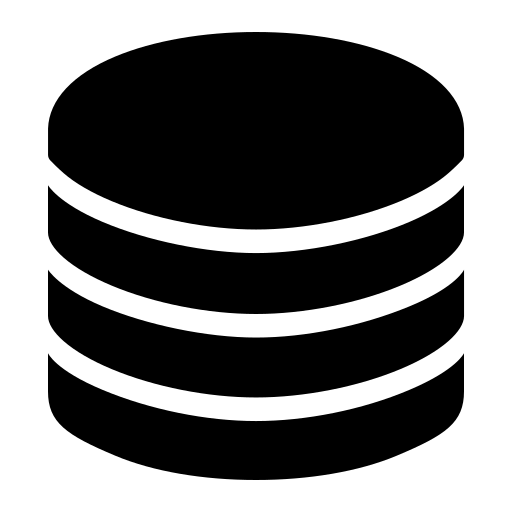
\includegraphics[height=0.9cm]{logos/CleanEasy-logo2.png}
    % };
    
    % 
    \node[anchor=north east, xshift=-0.8cm, yshift=-0.3cm] at (current page.north east) {
      
\includegraphics[height=2.2cm]{logos/logo_simee.png}
    };
    
    %
    % \node[anchor=north east, xshift=-2.8cm, yshift=-0.3cm] at (current page.north east) {
    %   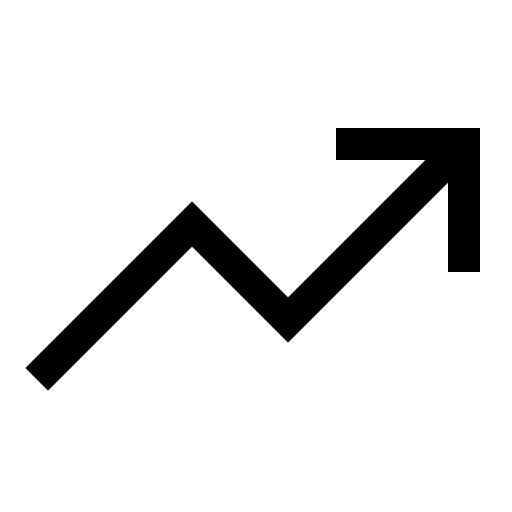
\includegraphics[height=1.4cm]{logos/CleanEasy-logo4.png}
    % };
  \end{tikzpicture}
}


%----------------------------------------------------------------------------------------

\newcommand{\prob}{\text{prob}}

\bibliography{reference}

\begin{document}

\begin{frame}[plain]
  \titlepage
\end{frame}

\begin{frame}[plain]{Conteúdos}
  \tableofcontents
\end{frame}

\section{Introdução}
\begin{frame}{Introdução}

\end{frame}

\section{Teorema de Bayes}
\begin{frame}{Teorema de Bayes}
Regras de probabilidade \footcite{Sivia_2006}:

\begin{align}
  \prob(X | I) &+ \prob(\bar X | I) = 1, \\
  \prob(X,Y | I) &= \prob(X | Y, I) \; \prob(Y | I). \label{probcond}
\end{align}

\end{frame}

\begin{frame}{Como entender probabilidades condicionais?}
  Imagine, por exemplo, que você tem uma com 3 bolas vermelhas e 4 azuis. Você retira uma bola e, sem ver qual foi a primeira a ser retirada, retira outra. Sabendo que a segunda bola é vermelha, qual é a probabilidade de que a primeira tenha sido azul?

  \begin{itemize}
    \item No caso limite onde temos uma bola vermelha e uma azul, a resposta é $1$.
    \item Podemos utilizar (\ref{probcond}) para calcular a probabilidade de que a primeira bola seja azul dado que a segunda é vermelha:
  \end{itemize}

  \begin{equation}
    \prob(A_1 | V_2) = \frac{12/42}{18/42} = \frac{2}{3}.
  \end{equation}

  \begin{itemize}
    \item \textbf{\emph{Não se trata de uma ligação causal!!}}
  \end{itemize}
\end{frame}

\begin{frame}
  Podemos então encontrar o teorema de Bayes quando reconhecemos que $\prob(X, Y | I) = \prob(Y, X | I)$:
  
  \begin{equation}
  \begin{aligned}
    \prob(X | Y, I) \prob(Y | I) &= \prob(Y | X, I) \prob(X | I), \\
    \prob(X | Y, I) &= \frac{\prob(Y | X, I) \prob(X | I)}{\prob(Y | I)}.
  \end{aligned}
  \end{equation}
\end{frame}

\begin{frame}{Caso contínuo}
  No caso contínuo, o teorema de Bayes segue o mesmo, apenas temos a normalização e marginalização da forma:
  
  \begin{equation}
  \begin{aligned}
    \int \prob(Y | I) dY &= 1, \\
    \int \prob(Y,X | I) dX &= \prob(Y | I).
  \end{aligned}
  \end{equation}
\end{frame}

\begin{frame}{Estimação de parâmetros}
  \begin{figure}
    \centering
    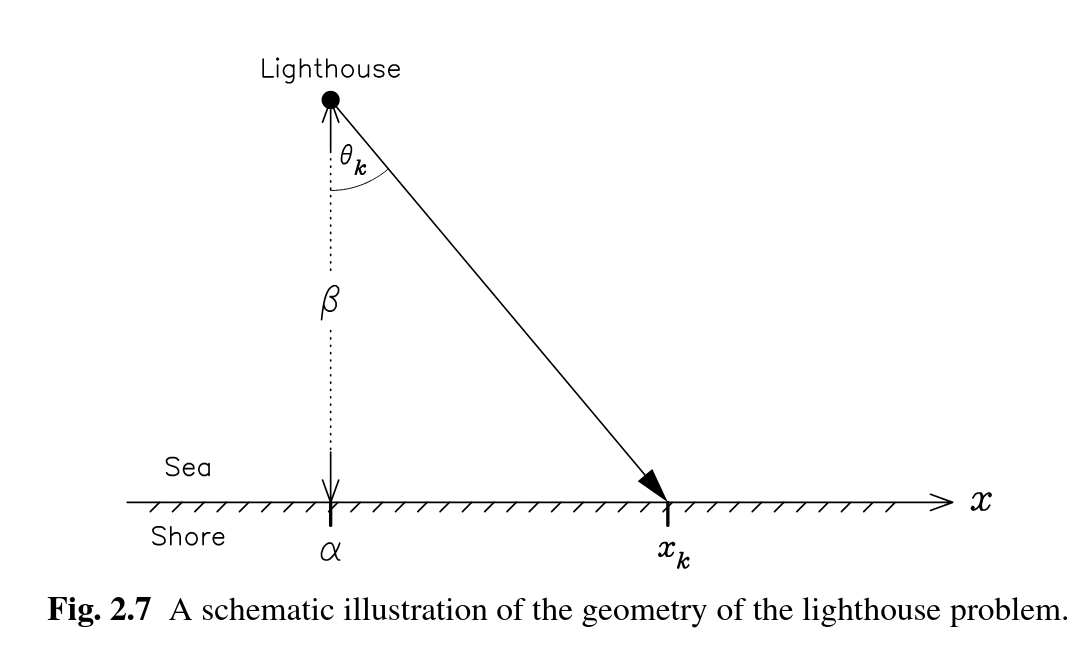
\includegraphics[width=0.6\textwidth]{farol.png}
    \caption{Esquemática de um problema com dois parâmetros: $\alpha$ e $\beta$ \footcite{Sivia_2006}.}
  \end{figure}
\end{frame}

\begin{frame}
  \begin{itemize}
    \item Para o caso analítico, vamos focar em apenas um dos parâmetros: a posição do farol na costa, $\alpha$, assumindo que sabemos a distância dele da costa, $\beta$.
  \end{itemize}

  Podemos definir o ângulo $\theta$ com

  \begin{equation}
    \beta \tan(\theta_k) = x_k - \alpha,
  \end{equation}

  Então definimos uma distribuição uniforme em $\theta$:

  \begin{equation}
    \prob(\theta | \alpha, \beta, I) = \frac{1}{\pi}
  \end{equation}

  Podemos obter uma distribuição e $x$:

  \begin{equation}
    \prob(x_k | \alpha, \beta, I) = \frac{\beta}{\pi \left[ \beta^2 + (x_k - \alpha)^2 \right]} 
  \end{equation}

  \emph{É uma distribuição de Cauchy (ou Lorentz(iana) ou de Breit-Wigner).}
\end{frame}

\begin{frame} 
  Utilizamos o teorema de Bayes:
  \begin{equation}
    \prob(\alpha | {x_k}, \beta, I) \propto \prob({x_k} | \alpha, \beta, I) \prob(\alpha | \beta, I)
  \end{equation}

  Com a distribuição inicial (prior)

  \begin{equation}
    \prob(\alpha | \beta, I) \sim \mathcal{U}(\alpha_\text{min}, \alpha_\text{max}),
  \end{equation}
  podemos atualizar nossa confiança da posição do farol ao longo da costa

  \begin{equation}
    \prob({x_k} | \alpha, \beta, I) = \prod_{k=1}^{N} \prob(x_k | \alpha, \beta, I)
  \end{equation}

  então obter a melhor estimativa da posição do farol $\alpha_0$ (segundo uma estimação de máximo a posteriori):

  \begin{equation}
    2 \sum_{k=1}^{N} \frac{x_k - \alpha_0}{\beta^2 + (x_k - \alpha_0)^2} = 0.
  \end{equation}
\end{frame}

\begin{equation}
  
\end{equation}

\begin{frame}{Referências}
  \printbibliography[heading=none] 
\end{frame}

\end{document}